%!TEX root = paper.tex
%%%%%%%%%%%%%%%%%%%%%%%%%%%%%%%%%%%%%%%%%%%%%%%%%%%%%%%%%%%%%%%%%%%%%%%%%%%%%%%%
\section{Lag Simulation}
\label{sec:simulation}

Based on the models introduced in Section~\ref{sec:model} a stochastic \textsc{Gnu R}-based \gls{DES} was created\footnote{\url{https://github.com/mas-ude/onlinegame-lag-sim/tree/master/simulation}}.

Due to the influence of several stochastic processes (user inputs $U$, network delay $D$, server processing time $P$) and the differing offset of the clocked processes, a sufficient number of repetitions is required to provide meaningful results. The investigations here are intended to highlight some particular aspect in each of the scenarios

Besides being fully reconfigurable, the simulation currently also has a few default parameters set and makes assumptions that go beyond what the base end-to-end model implies for reasons of simplicity.
%They are chosen to be as realistic as possible and and are summarized in Table~\ref{tab:notation}.
First, the input is modeled by an exponential distribution with a rate of $20$ events per second. The offsets between the clocked processes are uniformly distributed in their respective intervals. It is further assumed that the server processing time $P$ follows a left-truncated normal distribution with $\mu_P = \SI{3}{\milli\second}$ and $\sigma_P = \SI{0.1}{\milli\second}$. Additionally, the rate $c$ at which command messages are sent to the game server is set equal to the server's tickrate $g$ as the server would not process more commands either way. This might however increase the end-to-end lag in some situations if a command message just misses one of the server's ticks and has to wait another full cycle. The evaluation of the presented scenarios was conducted on the basis of $r=\np{1000}$ repetitions for each setting. Each run $i \in \{1,\dots,r\}$ consisted of a series of $n=\np{100}$ input events and their associated end-to-end lag $T_{i,j}$ for the $j$-th input event. On this basis a median lag $\widetilde{T_i}$ was calculated over the $n$ input events for each run $i$, and finally an overall mean lag out of the individiual medians of each repetition, i.e. $\overline{T}=\frac{1}{n}\sum_{i=1}^r\widetilde{T_i}$.


%%%%%%%%%%%%%%%%%%%%%%%%%%%%%%%%%%%%%%%%%%%%%%%%%%%%%%%%%%%%%%%%%%%%%%%%%%%%%%%%
\subsection{Basic Game Results}


Looking at typical \SI{60}{\hertz} local games (i.e. a frame duration of $\approx \SI{16.6}{\milli\second}$) the median lag is \SIrange{45}{50}{\milli\second}. So even under quasi-optimal circumstances, there is already a considerable amount of \gls{E2E} lag (even without factoring in the delay of the screen and input devices) caused by the interactions of several random and clocked processes. Higher framerates alleviate this somewhat.


\begin{figure}[!t]
	\centering
	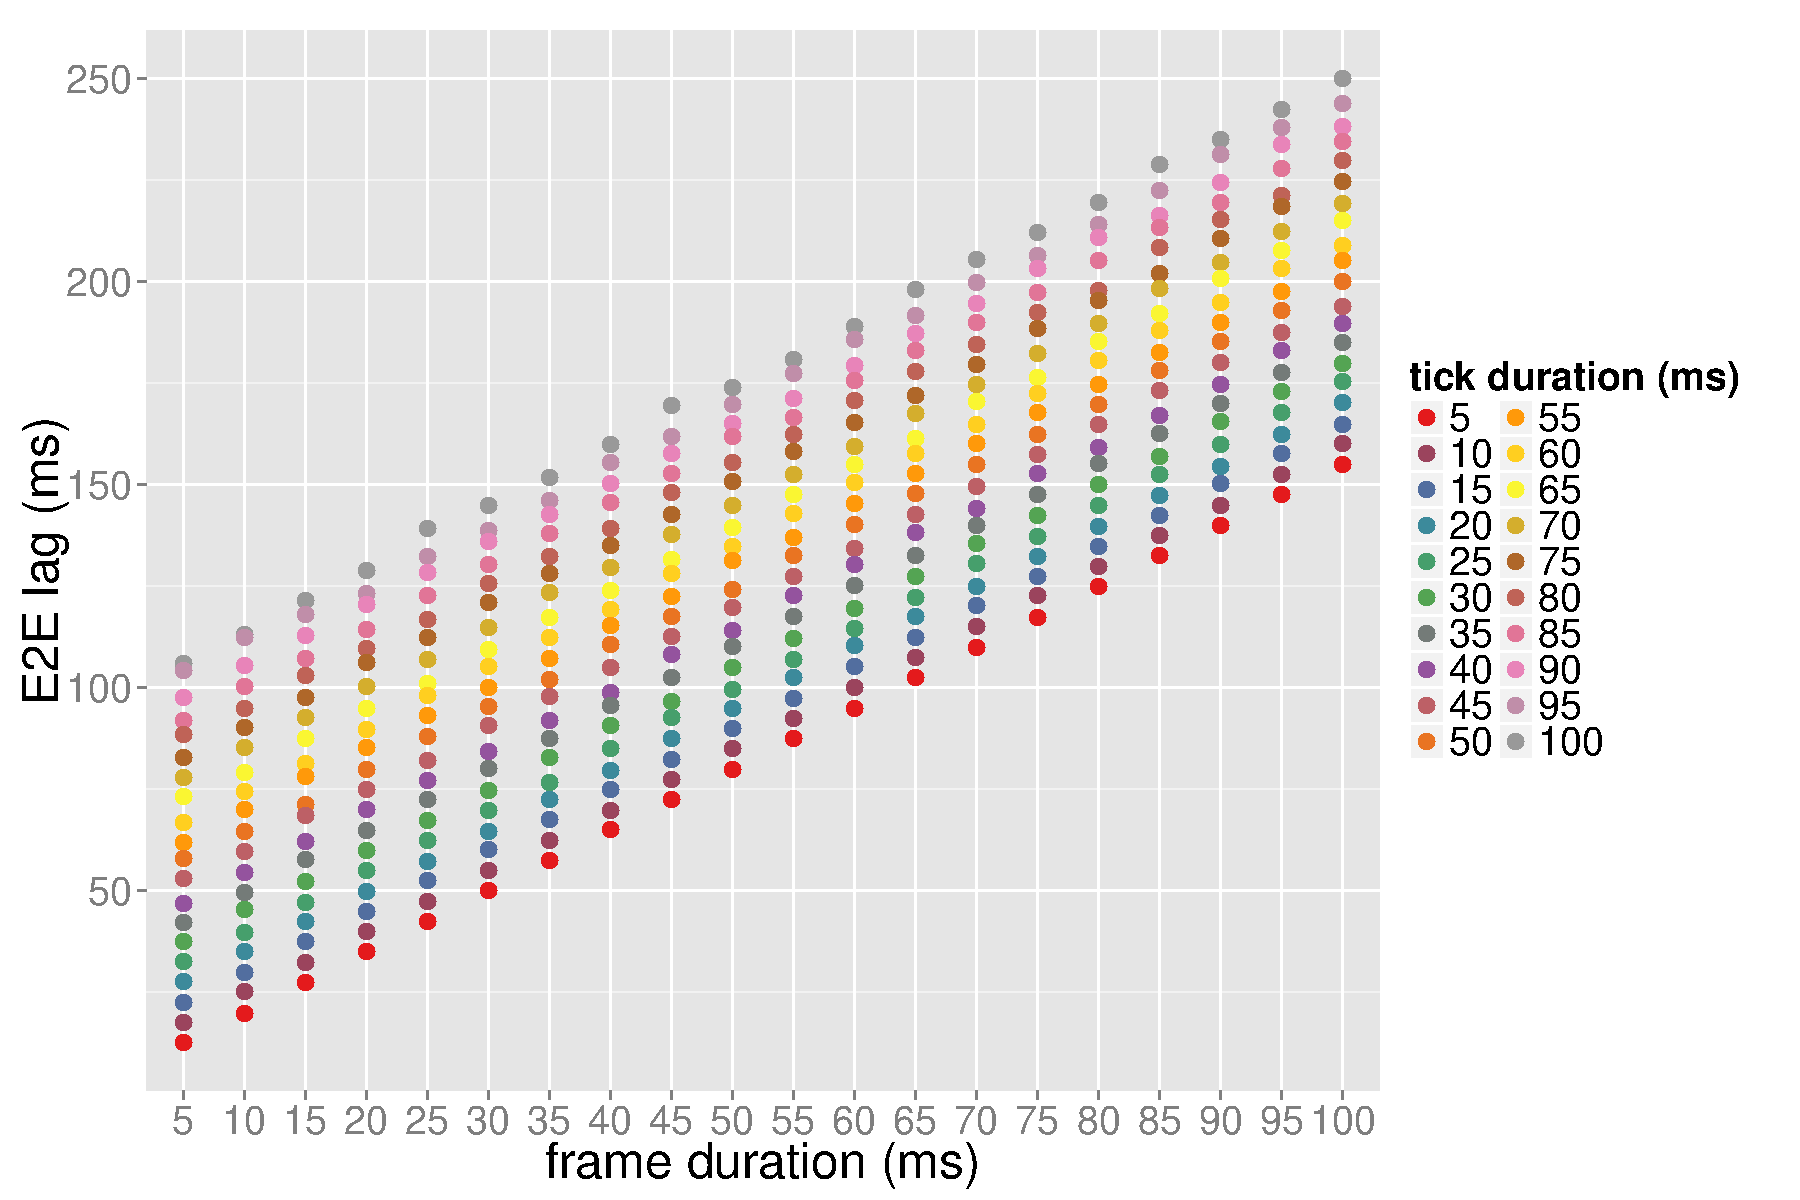
\includegraphics[width=1.0\columnwidth]{../../../simulation/visualization/nwless-onlinegame-1000rounds.pdf}
	\caption{Median end-to-end lag under various frame and tick durations for a locally-running game. Lower lag values are achieved at lower frame and tick durations.}
\label{fig:nwless-scatter}
\end{figure}

The first and simplest scenario to be investigated here is the case of the local game. In the version implemented here, the tickrate is still present, but the influence of the network is entirely removed. It therefore represents the best case an online multiplayer game could achieve if the server ran locally. Figure~\ref{fig:nwless-scatter} plots the relationship between the frame duration (i.e., the inverse of the framerate), the tick duration, and the resulting median end-to-end lag. The values can be estimated as follows. Every user input event traverses three queues with fixed-rate outputs ($c=g$, g, and $f$), and every game state update waits for the next full frame until it gets displayed. In the ideal case, an input event occurs just before the command message is sent off, the server tick follows as soon as the message is received, and the update reaches the client just before a frame is output. Then the end-to-end lag is slightly above the frame time that must elapse before the update can be rendered to screen, $T_{min}>f^{-1}$. In case the events are unfavorably offset against one another, an input event has to wait almost a full command-message cycle until it is sent on; it reaches the server just after a tick has occurred, so it waits almost a full server tick; finally, it will wait for almost two frame times until it is displayed. Combining with the previous result bounds the lag as follows, $f^{-1} < T < c^{-1}+g^{-1}+2f^{-1}$. The mid-interval point between these two limits is $T_{mid}=\frac{3}{2} f^{-1} + g^{-1}|_{c=g}$ which coincides roughly with the medians of the stochastic simulation. Looking at a typical \SI{60}{\hertz} video game with an equal tickrate (i.e. a frame duration of $\approx \SI{16.6}{\milli\second}$) the median lag is in the range of \SIrange{45}{50}{\milli\second}. So even under quasi-optimal circumstances, there is already a considerable amount of end-to-end lag (even without factoring in the delay of the screen and input devices) that can only increase with the presence of network delay. Therefore, video games (and quality assessments thereof) should try to achieve the highest framerate possible to minimize this influence.

%%%%%%%%%%%%%%%%%%%%%%%%%%%%%%%%%%%%%%%%%%%%%%%%%%%%%%%%%%%%%%%%%%%%%%%%%%%%%%%%
\subsection{Online Gaming}


 In the online scenario the framerate has a larger influence on the lag than the tickrate. For low framerates and tickrates, the impact of network delay on the \gls{E2E} lag is almost completely masked. Only if both rates are high enough, the network delay will play a more significant role. This masking effect has large implications for video games and their evaluation. Many evaluations examine the influence of the network delay without considering other contributions to the \gls{E2E} lag. These results indicate that this might not be the best course of action. The effect likely shifts to lower values of the frame- and tickrates when a higher network delay is examined.


% \begin{figure}[!t]
% 	\centering
% 	\vspace{-6mm}
% 	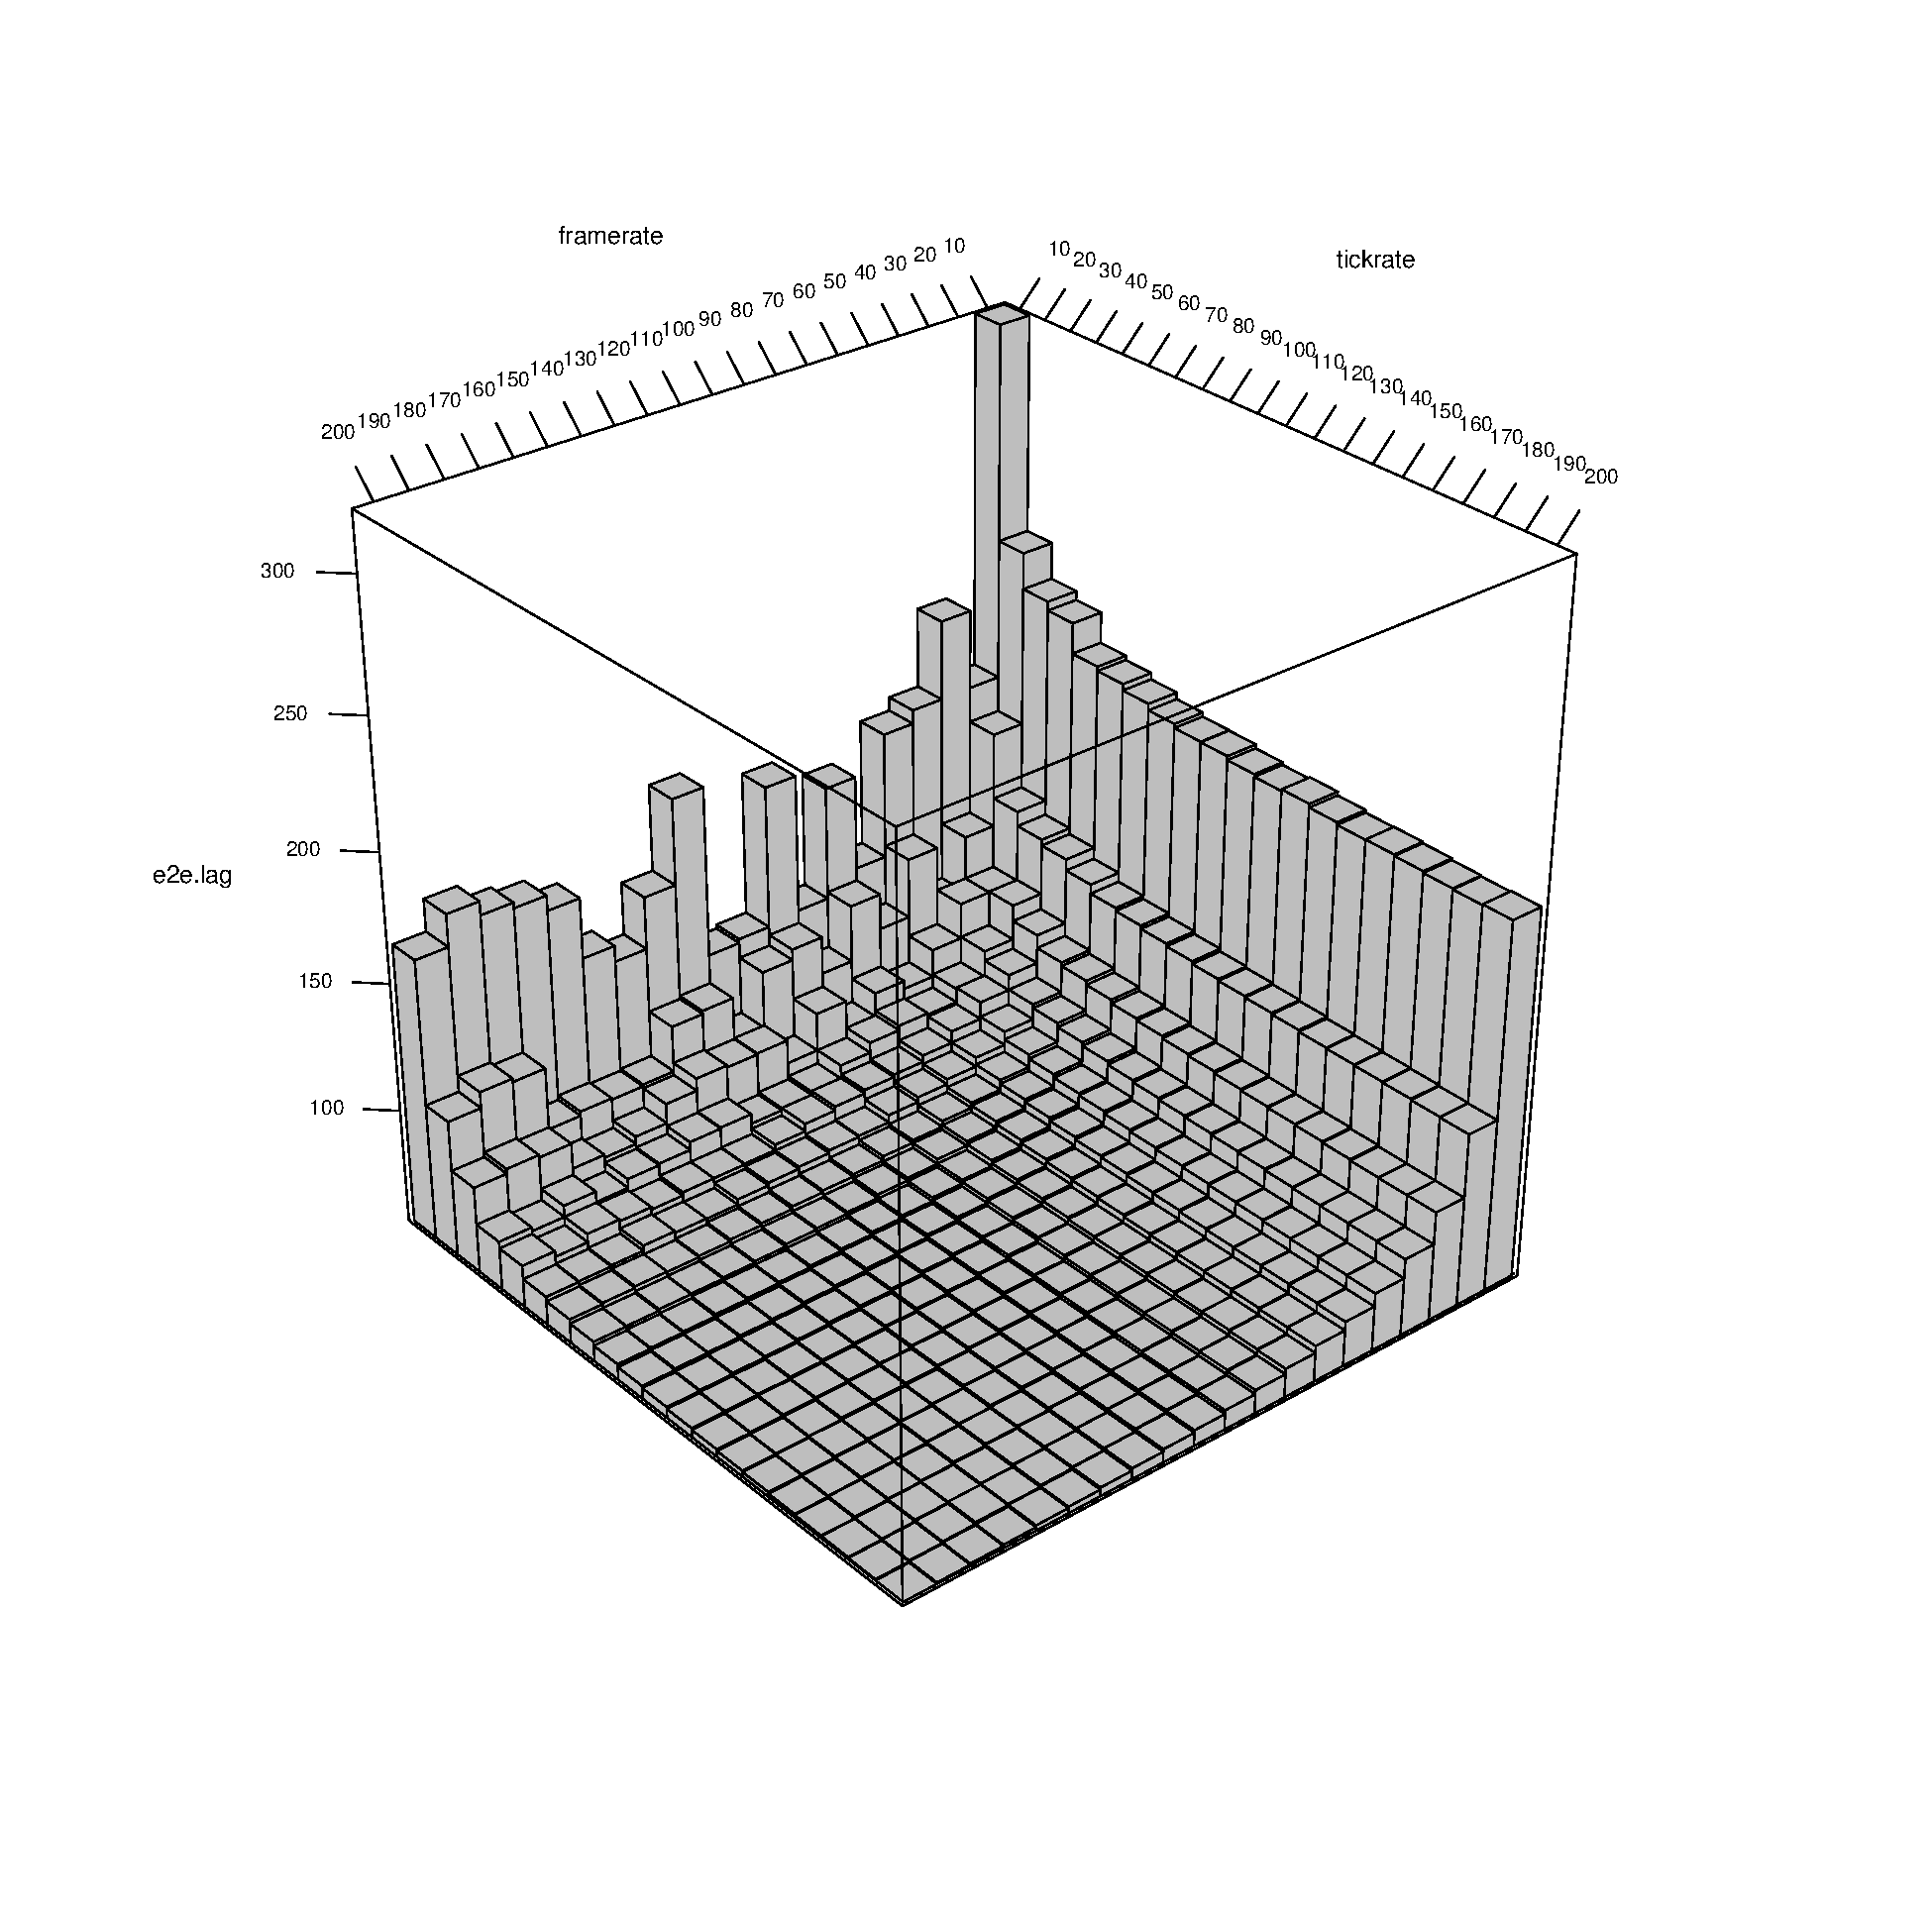
\includegraphics[width=1.0\columnwidth]{../../../simulation/visualization/e2e-lag-3dbars.pdf}
% 	\vspace{-15mm}
% 	\caption{Influence of client framerate and server tickrate on the median end-to-end lag in the online game scenario. For high rates $f$, $g$, the lag approaches $2\mu_D+\mu_P=\SI{43}{\milli\second}$.}
% \label{fig:3dbars-framerate-tickrate-lag}
% \end{figure}

Next up is the full scenario of an online video game, now with network lag $D$ and server processing time $P$ included. For this exemplary scenario, the one-way delay $D$ was assumed to follow a left-truncated normal distribution, with $\mu_D = \SI{20}{\milli\second}$ and $\sigma_D = \SI{5}{\milli\second}$, producing non-negative network delays. Typical competitive online games today are expected to operate in such ranges. An \acrshort{RTT} of \SI{100}{\milli\second} is often considered to be the upper limit for a good playing experience. $P$ is similarly left-truncated. In addition to the components in the previous scenario, the lag now also contains contributions by the network round-trip and processing delay, $2D + P$.

%Figure~\ref{fig:3dbars-framerate-tickrate-lag} shows a 3D bar plot of the influence of both the framerate and the tickrate on this scenario. The axes mark typical values for $f$ and $g$. 
Two things can be noted of the influence of frame and tickrates in this scenario. First, the framerate has a larger influence on the lag than the tickrate. Second, for low framerates and tickrates, the impact of network delay on the end-to-end lag is almost completely masked. Only if both rates are high enough, the network delay will play a more significant role. This masking effect has large implications for video games and their evaluation. Many evaluations examine the influence of the network delay only, without considering other contributions to end-to-end lag. Our results indicate that this might not be the best course of action. The effect likely shifts to lower values of the frame- and tickrates when a higher network delay is examined. %Another interesting result (not plotted here) is the much larger variance of lag in the framerate dimension when compared to the tickrate. This requires video game studies to have a very high repetition rate to provide meaningful results.


%%%%%%%%%%%%%%%%%%%%%%%%%%%%%%%%%%%%%%%%%%%%%%%%%%%%%%%%%%%%%%%%%%%%%%%%%%%%%%%%
\subsection{Cloud Gaming}

 In the Cloud Gaming scenario in Fig.~\ref{fig:cloud-e2e-delay-sim}, the network delay is set to \SI{40}{\milli\second} (average round-trip); it is seen that the framerate impacts the \gls{E2E} lag more severely than the network does. This result is of particular importance considering how past studies have relied on similarly low framerates as $5-\SI{15}{\hertz}$ when assessing the network influence on cloud gaming. Similarly, our results can provide guidelines for implementors of cloud gaming to factor in the framerate in their calculations accordingly.


\begin{figure}[!t]
	\centering
	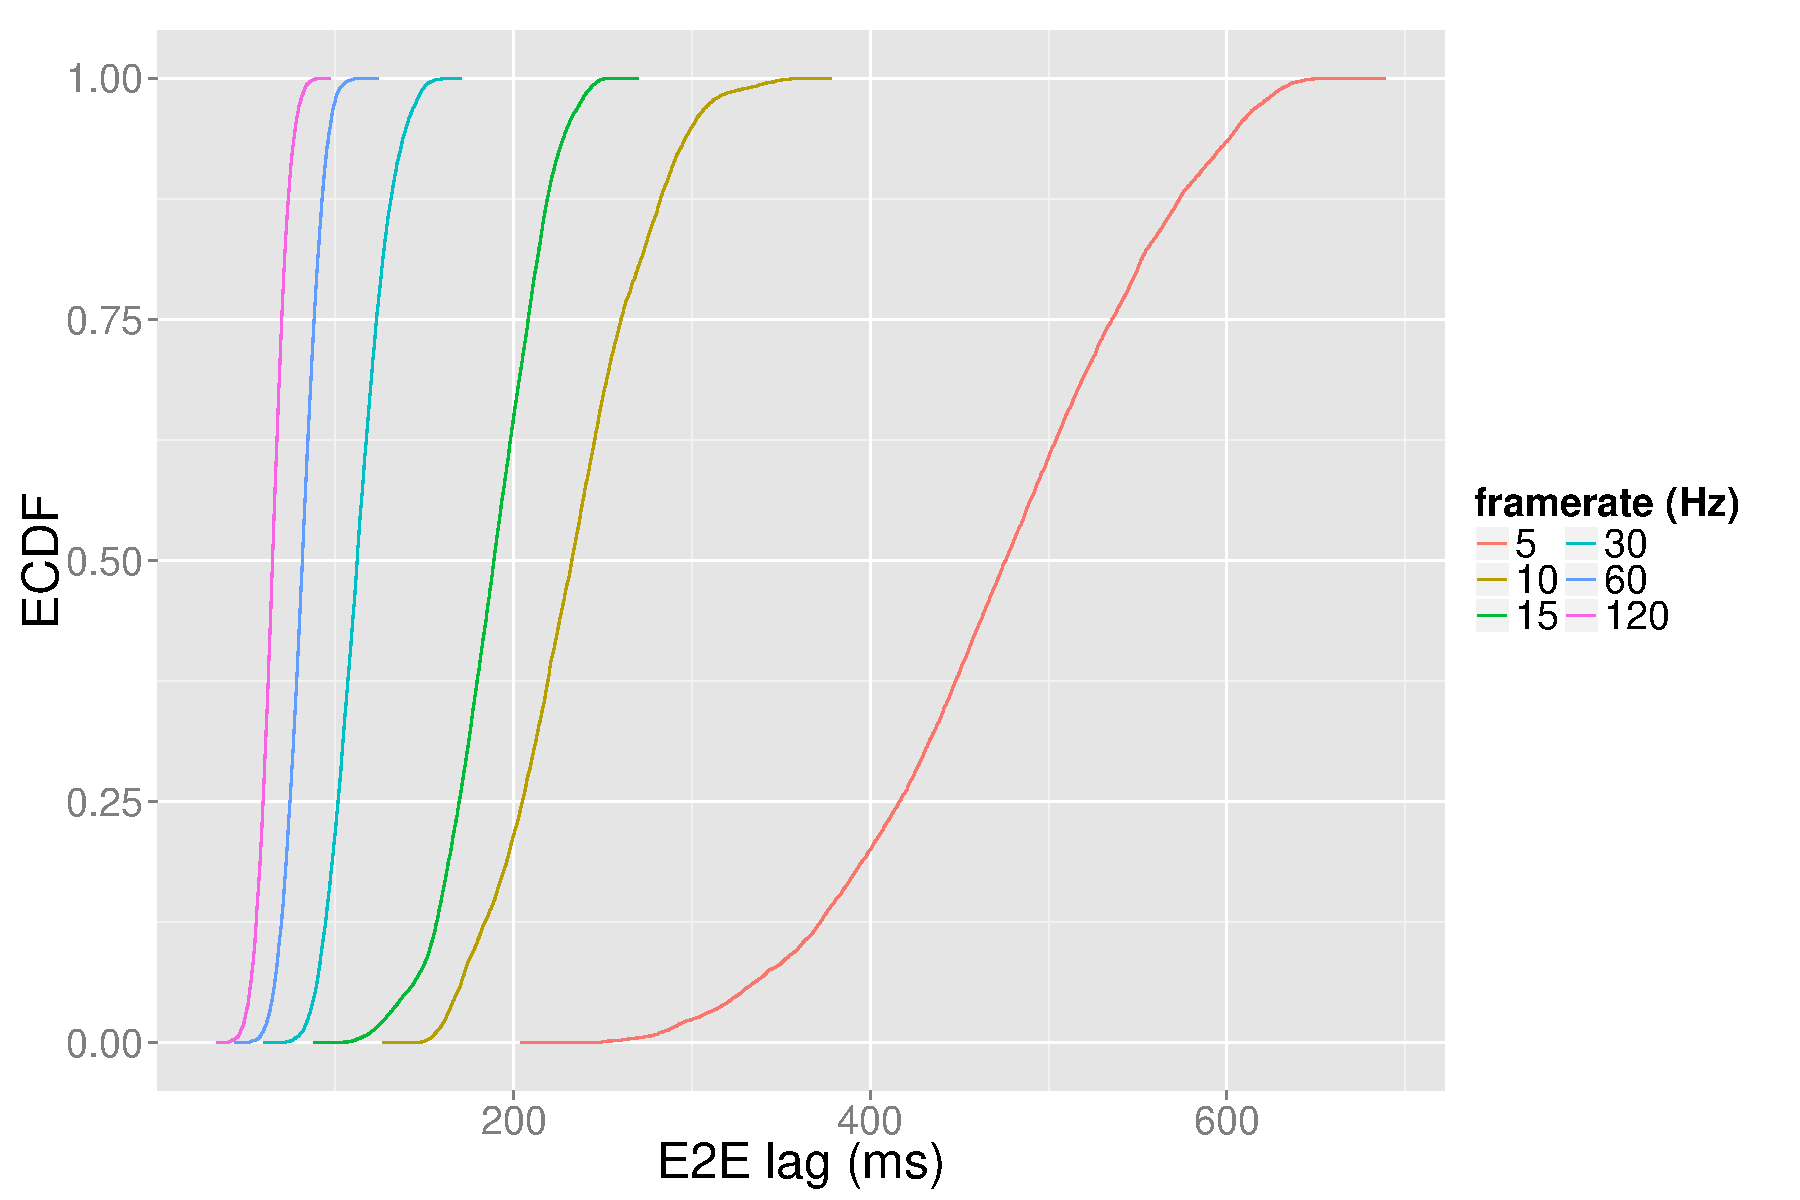
\includegraphics[width=1.0\columnwidth]{../../../simulation/visualization/cloudgaming-lag-cdf.pdf}
	\caption{Influence of the rendering and streaming framerate on the \gls{E2E} lag in the cloud scenario. Vertical intercept denotes the average server, network and codec delay of \SI{68}{\milli\second}.}
\label{fig:cloud-e2e-delay-sim}
\end{figure}

Finally, we construct a Cloud Gaming scenario. The tickrate has been removed;  instead, a constant encode ($e$) and decode ($d$) delay is in place at the game streaming server and client respectively. The frames are now rendered by the server, so they need to be transported back to the client first. Instead of assuming a specific network throughput and frame size, we simply add one frame time to account for the transmission of the encoded screen contents. For the network delay $D$, the same values as for the online game are used. $c$ is set to $\SI{200}{\hertz}$. Figure~\ref{fig:cloud-e2e-delay-sim} shows the results of this scenario as an \gls{ECDF} of the end-to-end lag for several framerates. As before, the framerate impacts the end-to-end lag more severely than the network delay. This result is of particular importance considering how past studies have relied on similarly low framerates as $5-\SI{15}{\hertz}$ when assessing the network influence on cloud gaming. Similarly, these results can provide guidelines for implementors of cloud gaming to factor in the framerate in their calculations accordingly.

